\chapter{Технологическая часть}

В данном разделе рассматриваются средства реализации программного комплекса, структура разработанного приложения, особенности физической реализации базы данных, организация конфигурирования и логирования, реализация графического интерфейса, ролевой модели, триггеров, функций и кэширования.

\section{Выбор средств реализации}

В качестве основной системы управления базами данных была выбрана PostgreSQL. Данная СУБД поддерживает транзакции, внешние ключи, ограничения целостности, индексы, пользовательские функции, триггеры и развитую ролевую модель, что необходимо для реализации системы хранения и обработки стоматологических снимков~\cite{postgresql_docs}.

Для реализации серверной логики приложения был выбран язык C++17. Выбор обусловлен возможностью строгой типизации доменных сущностей, явного управления зависимостями компонентов и наличием библиотек для работы с PostgreSQL, Redis, логированием и графическим интерфейсом.

Для доступа к PostgreSQL используется библиотека \texttt{libpqxx}, являющаяся C++-обёрткой над клиентской библиотекой PostgreSQL. Она позволяет выполнять SQL-запросы, работать с транзакциями и получать результаты запросов в типизированном виде~\cite{libpqxx_docs}.

Для реализации графического интерфейса была выбрана библиотека Qt 6. Qt предоставляет набор виджетов для построения оконных приложений, механизм сигналов и слотов, а также средства компоновки элементов интерфейса \cite{qt_docs}. Графический интерфейс реализован отдельным компонентом и взаимодействует с системой через общий интерфейс прикладной логики.

Для логирования используется библиотека \texttt{spdlog}. Она поддерживает различные уровни логирования, запись сообщений в файл и настройку формата вывода \cite{spdlog_docs}. В проекте библиотека используется через собственный компонент-обёртку \texttt{Logger}, что позволяет не связывать остальные компоненты напрямую с внешней библиотекой.

Для кэширования используется Redis. Redis выбран как In-Memory СУБД, позволяющая хранить часто запрашиваемые данные в оперативной памяти и уменьшать количество обращений к основной реляционной базе данных \cite{redis_docs}. Взаимодействие с Redis выполняется через библиотеку \texttt{hiredis}.

Сборка проекта выполняется с использованием CMake. Данный инструмент позволяет описывать структуру проекта, зависимости между компонентами, параметры компиляции и правила формирования исполняемых файлов и статических библиотек \cite{cmake_docs}.

\section{Структура программного комплекса}

Разработанное приложение построено по компонентному принципу. Каждый логический компонент оформлен в виде отдельной программной сборки. Такой подход соответствует требованию разделения компонентов как единиц развёртывания.

В проекте выделены следующие основные компоненты:

\begin{itemize}
	\item \texttt{dentobase\_config} --- компонент чтения конфигурационных файлов;
	\item \texttt{dentobase\_logging} --- компонент логирования на основе \texttt{spdlog};
	\item \texttt{dentobase\_cache} --- компонент Redis-кэширования;
	\item \texttt{dentobase\_data\_access} --- компонент доступа к PostgreSQL;
	\item \texttt{dentobase\_business} --- компонент бизнес-логики;
	\item \texttt{dentobase\_gui} --- компонент графического интерфейса;
	\item \texttt{dentobase\_gui\_app} --- исполняемый файл приложения.
\end{itemize}

Компоненты собираются в виде статических библиотек, после чего связываются с исполняемым файлом приложения. Директория с результатами сборки содержит отдельные файлы компонентов, что позволяет явно продемонстрировать компонентную структуру приложения.

\section{Конфигурирование приложения}

Параметры, зависящие от окружения запуска, вынесены в конфигурационные файлы. Такой подход позволяет изменять параметры подключения к базе данных, Redis и логированию без перекомпиляции приложения.

Пример конфигурационного файла приведён в листинге~\ref{lst:admin-config}.

\clearpage

\begin{lstlisting}[caption={Пример конфигурационного файла администратора}, label={lst:admin-config}]
	db.connection_string=host=127.0.0.1 port=5432 dbname=dentobase_test user=dentobase_admin_user password=admin_password
	log.file=logs/admin.log
	log.level=debug
	
	redis.enabled=true
	redis.host=127.0.0.1
	redis.port=6379
	redis.ttl_seconds=300
	
	business.max_diagnosis_text_length=2048
\end{lstlisting}

В проекте предусмотрены отдельные конфигурационные файлы для разных ролей:

\begin{itemize}
	\item \texttt{admin.conf} --- запуск приложения от имени администратора;
	\item \texttt{doctor.conf} --- запуск приложения от имени врача;
	\item \texttt{technician.conf} --- запуск приложения от имени лаборанта;
	\item \texttt{app.conf} --- технический конфигурационный файл для запуска от имени пользователя PostgreSQL.
\end{itemize}

Чтение параметров выполняется компонентом \texttt{Config}. Конфигурационный файл имеет формат \texttt{key=value}. При запуске приложения путь к конфигурационному файлу передаётся через аргументы командной строки.

\section{Логирование}

Логирование реализовано с использованием библиотеки \texttt{spdlog}. Для изоляции внешней библиотеки от остальной части системы создан компонент \texttt{Logger}. Остальные компоненты используют только методы \texttt{debug}, \texttt{info}, \texttt{warning} и \texttt{error}.

Поддерживаются следующие уровни логирования:

\begin{itemize}
	\item \texttt{DEBUG} --- подробные отладочные сообщения;
	\item \texttt{INFO} --- основные действия пользователя и этапы работы приложения;
	\item \texttt{WARNING} --- нефатальные ошибки и нестандартные ситуации;
	\item \texttt{ERROR} --- исключительные ситуации, препятствующие выполнению операции.
\end{itemize}

Уровень логирования задаётся в конфигурационном файле. Для режима \texttt{debug} записываются все сообщения, включая отладочные. Для режима \texttt{release} сообщения уровня \texttt{DEBUG} не записываются.

В лог-файл записываются:

\begin{itemize}
	\item запуск и завершение приложения;
	\item путь к используемому конфигурационному файлу;
	\item подключение к PostgreSQL;
	\item подключение к Redis;
	\item действия пользователя в графическом интерфейсе;
	\item ошибки выполнения операций;
	\item события попадания и промаха Redis-кэша.
\end{itemize}

\section{Физическая реализация базы данных}

Физическая схема базы данных реализована в файле \texttt{database/schema.sql}. В базе данных созданы таблицы:

\begin{itemize}
	\item \texttt{patients} --- пациенты;
	\item \texttt{clinics} --- клиники;
	\item \texttt{doctors} --- врачи;
	\item \texttt{doctor\_clinics} --- связь врачей и клиник;
	\item \texttt{technicians} --- лаборанты;
	\item \texttt{equipment} --- оборудование;
	\item \texttt{image\_types} --- типы снимков;
	\item \texttt{medical\_records} --- медицинские карты;
	\item \texttt{images} --- стоматологические снимки;
	\item \texttt{diagnoses} --- заключения врачей.
\end{itemize}

Для идентификации записей используется тип \texttt{UUID}. Для хранения бинарных данных снимков используется тип \texttt{BYTEA}. Связи между таблицами реализованы с помощью внешних ключей.

Связь между врачами и клиниками является связью многие-ко-многим. Она реализована через промежуточную таблицу \texttt{doctor\_clinics}, содержащую пары идентификаторов врача и клиники.

Фрагмент схемы связи многие-ко-многим приведён в листинге~\ref{lst:doctor-clinics}.

\begin{lstlisting}[caption={Реализация связи многие-ко-многим между врачами и клиниками}, label={lst:doctor-clinics}]
	CREATE TABLE doctor_clinics (
	doctor_id UUID NOT NULL REFERENCES doctors(id) ON DELETE CASCADE,
	clinic_id UUID NOT NULL REFERENCES clinics(id) ON DELETE CASCADE,
	PRIMARY KEY (doctor_id, clinic_id)
	);
\end{lstlisting}

\section{Инициализация базы данных}

Для автоматизации развёртывания базы данных разработан скрипт \texttt{reset.sh}. Скрипт выполняет полный цикл пересоздания базы данных:

\begin{enumerate}
	\item запуск контейнеров PostgreSQL и Redis;
	\item ожидание готовности PostgreSQL;
	\item удаление существующей базы данных;
	\item создание новой базы данных \texttt{dentobase\_test};
	\item применение схемы \texttt{schema.sql};
	\item применение функций \texttt{functions.sql};
	\item применение триггеров \texttt{triggers.sql};
	\item генерация тестовых данных;
	\item применение ролевой модели;
	\item проверка количества записей в таблицах.
\end{enumerate}

Таким образом, для подготовки рабочей базы данных достаточно выполнить команду:

\begin{lstlisting}[caption={Полное пересоздание базы данных}]
	./scripts/reset.sh
\end{lstlisting}

Для генерации тестовых данных используется скрипт \texttt{generate\_seed.py}. Он формирует файл \texttt{database/seed.sql}, содержащий не менее 1000 записей для каждой таблицы. После применения данных выполняется контроль количества строк.

\section{Ролевая модель базы данных}

В PostgreSQL реализована ролевая модель доступа. Используются три основные роли:

\begin{itemize}
	\item \texttt{dentobase\_admin} --- администратор;
	\item \texttt{dentobase\_doctor} --- врач;
	\item \texttt{dentobase\_technician} --- лаборант.
\end{itemize}

Для каждой роли создан отдельный пользователь базы данных:

\begin{itemize}
	\item \texttt{dentobase\_admin\_user};
	\item \texttt{dentobase\_doctor\_user};
	\item \texttt{dentobase\_technician\_user}.
\end{itemize}

Администратор имеет полный доступ ко всем таблицам. Врач имеет доступ к просмотру медицинских данных и созданию заключений. Лаборант имеет доступ к созданию пациентов, медицинских карт и снимков, а также к просмотру справочников.

Ролевая модель применяется скриптом \texttt{database/roles.sql}. Для запуска приложения под разными ролями используются разные конфигурационные файлы. Это позволяет проверять права доступа непосредственно через приложение.

\section{Функции и триггеры базы данных}

Для переноса части логики на сторону базы данных реализованы пользовательские функции и триггеры.

В файле \texttt{database/functions.sql} реализована функция получения снимков пациента. Она принимает идентификатор пациента и возвращает список связанных снимков с метаданными.

Общий вид функции приведён в листинге~\ref{lst:get-patient-images}.

\clearpage

\begin{lstlisting}[caption={Функция получения снимков пациента}, label={lst:get-patient-images}]
	CREATE OR REPLACE FUNCTION get_patient_images(p_patient_id UUID)
	RETURNS TABLE (
	image_id UUID,
	upload_date TIMESTAMP,
	image_type TEXT,
	equipment_model TEXT
	)
	AS $$
	BEGIN
	RETURN QUERY
	SELECT
	i.id,
	i.upload_date,
	it.name,
	e.model
	FROM images i
	JOIN image_types it ON it.id = i.type_id
	JOIN equipment e ON e.id = i.equip_id
	WHERE i.patient_id = p_patient_id
	ORDER BY i.upload_date DESC;
	END;
	$$ LANGUAGE plpgsql;
\end{lstlisting}

В файле \texttt{database/triggers.sql} реализован триггер обновления поля \texttt{updated\_at} в таблице медицинских карт. При изменении записи медицинской карты поле \texttt{updated\_at} автоматически устанавливается в текущее время.

Общий вид триггера приведён в листинге~\ref{lst:update-trigger}.

\clearpage

\begin{lstlisting}[caption={Триггер автоматического обновления времени изменения медицинской карты}, label={lst:update-trigger}]
	CREATE OR REPLACE FUNCTION update_medical_record_updated_at()
	RETURNS TRIGGER AS $$
	BEGIN
	NEW.updated_at = NOW();
	RETURN NEW;
	END;
	$$ LANGUAGE plpgsql;
	
	CREATE TRIGGER trg_update_medical_record_updated_at
	BEFORE UPDATE ON medical_records
	FOR EACH ROW
	EXECUTE FUNCTION update_medical_record_updated_at();
\end{lstlisting}

Использование триггера позволяет гарантировать корректность технического поля \texttt{updated\_at} независимо от того, каким способом была изменена запись.

\section{Компонент доступа к данным}

Доступ к базе данных реализован через слой репозиториев. Для каждой основной сущности создан интерфейс репозитория и реализация для PostgreSQL.

В проекте используются следующие репозитории:

\begin{itemize}
	\item \texttt{IPatientRepository} и \texttt{PostgresPatientRepository};
	\item \texttt{IDoctorRepository} и \texttt{PostgresDoctorRepository};
	\item \texttt{IMedicalRecordRepository} и \texttt{PostgresMedicalRecordRepository};
	\item \texttt{IImageRepository} и \texttt{PostgresImageRepository};
	\item \texttt{IDiagnosisRepository} и \texttt{PostgresDiagnosisRepository}.
\end{itemize}

Для отделения формирования SQL-запросов от выполнения запросов используются SQL-builder-ы. Это позволяет не смешивать код доступа к базе данных и код генерации SQL-строк.

Все операции изменения данных выполняются внутри транзакций. В случае успешного выполнения вызывается \texttt{commit}. При возникновении исключения транзакция отменяется автоматически.

\section{Компонент бизнес-логики}

Бизнес-логика сосредоточена в компоненте \texttt{dentobase\_business}. Основным входом в прикладной слой является интерфейс \texttt{IApplicationService}. Через данный интерфейс графический интерфейс выполняет все пользовательские сценарии.

В компоненте бизнес-логики реализованы следующие сценарии:

\begin{itemize}
	\item создание и поиск пациента;
	\item создание медицинской карты;
	\item создание, поиск и удаление клиник;
	\item создание, поиск и удаление врачей;
	\item создание, поиск и удаление лаборантов;
	\item создание, поиск и удаление оборудования;
	\item создание, поиск и удаление типов снимков;
	\item загрузка и поиск снимков;
	\item создание, поиск и удаление заключений;
	\item просмотр отдельных справочников.
\end{itemize}

Компонент бизнес-логики не зависит от графического интерфейса. Это позволяет при необходимости заменить интерфейс пользователя без изменения прикладных сценариев и слоя доступа к данным.

\section{Redis-кэширование}

Для уменьшения числа повторных обращений к PostgreSQL реализовано кэширование данных пациента в Redis. Кэширование оформлено отдельным компонентом \texttt{dentobase\_cache}.

Кэш работает через интерфейс \texttt{ICache}. Реализация \texttt{RedisCache} использует библиотеку \texttt{hiredis}. В конфигурационном файле задаются параметры подключения к Redis и время жизни записи в кэше.

При поиске пациента выполняется следующий алгоритм:

\begin{enumerate}
	\item формируется ключ вида \texttt{patient:<uuid>};
	\item выполняется попытка чтения значения из Redis;
	\item при наличии значения фиксируется \texttt{cache hit}, данные десериализуются и возвращаются в приложение;
	\item при отсутствии значения фиксируется \texttt{cache miss};
	\item данные читаются из PostgreSQL;
	\item полученный пациент сериализуется и помещается в Redis с заданным временем жизни.
\end{enumerate}

При создании нового пациента данные также записываются в Redis. Таким образом, повторный поиск созданного пациента может быть выполнен без обращения к основной базе данных.

\section{Графический интерфейс}

Графический интерфейс реализован с использованием Qt 6. Основным классом интерфейса является \texttt{MainWindow}. Интерфейс построен на основе вкладок, каждая из которых соответствует отдельной группе пользовательских сценариев.

В приложении реализованы следующие вкладки:

\begin{itemize}
	\item пациенты;
	\item медицинские карты;
	\item клиники;
	\item врачи;
	\item лаборанты;
	\item оборудование;
	\item типы снимков;
	\item снимки;
	\item заключения;
	\item справочники.
\end{itemize}

Для справочников реализован отдельный режим просмотра: пользователь выбирает нужный справочник из выпадающего списка, после чего данные отображаются в отдельном табличном окне. Такой подход удобнее, чем вывод всех справочников единым текстовым блоком.

Операции поиска и удаления реализованы для клиник, врачей, лаборантов, оборудования, типов снимков и заключений. Для опасных операций удаления используются отдельные кнопки, визуально выделенные красным цветом.

Графический интерфейс не обращается к базе данных напрямую. Все операции выполняются через \texttt{IApplicationService}. Это обеспечивает соблюдение принципа инверсии зависимостей и исключает дублирование бизнес-логики в интерфейсе.

Основные примеры взаимодействия с графическим интерфейсом представлены на рисунках \ref{fig:graph1} -- \ref{fig:graph4}.

\begin{figure}[H]
	\centering
	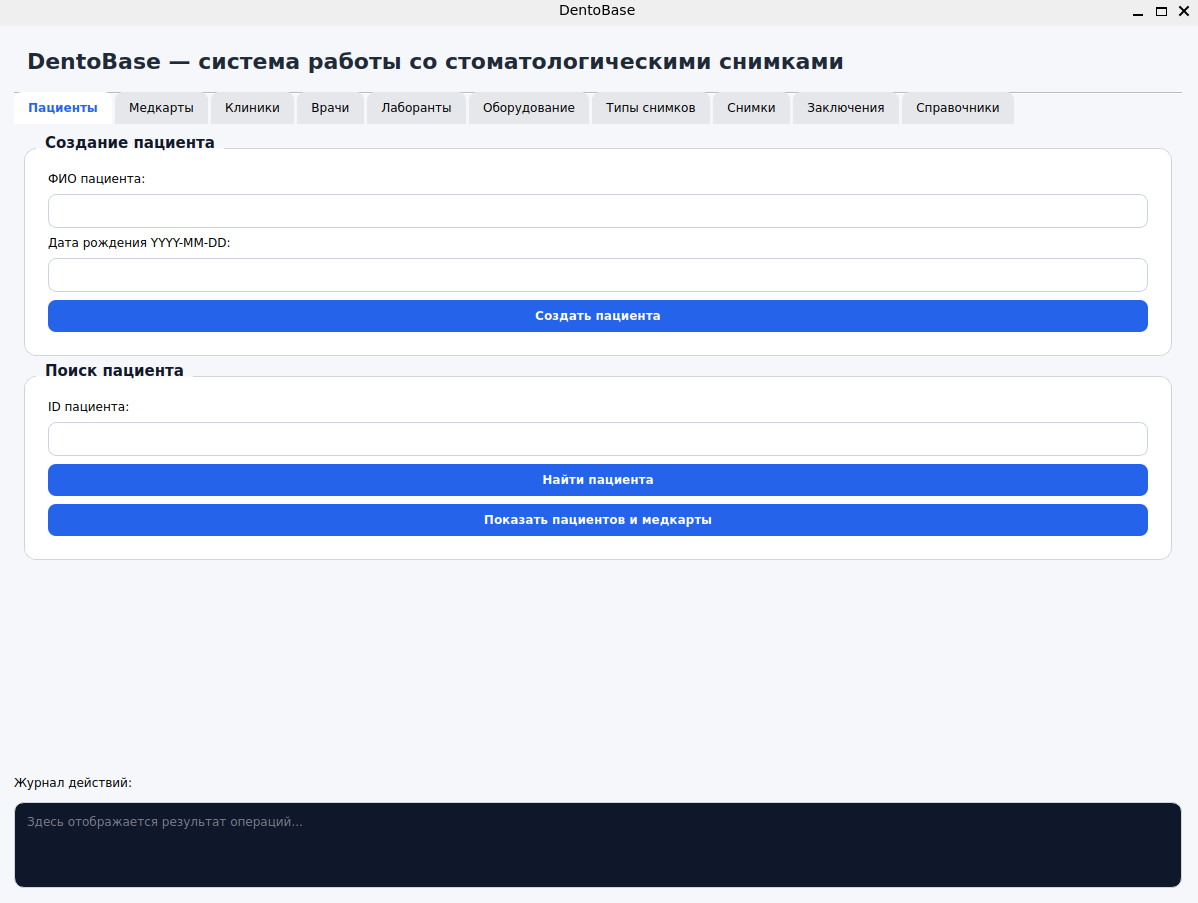
\includegraphics[width=0.7\textwidth]{graph1}
	\caption{Общий вид графического окна}
	\label{fig:graph1}
\end{figure}

\begin{figure}[H]
	\centering
	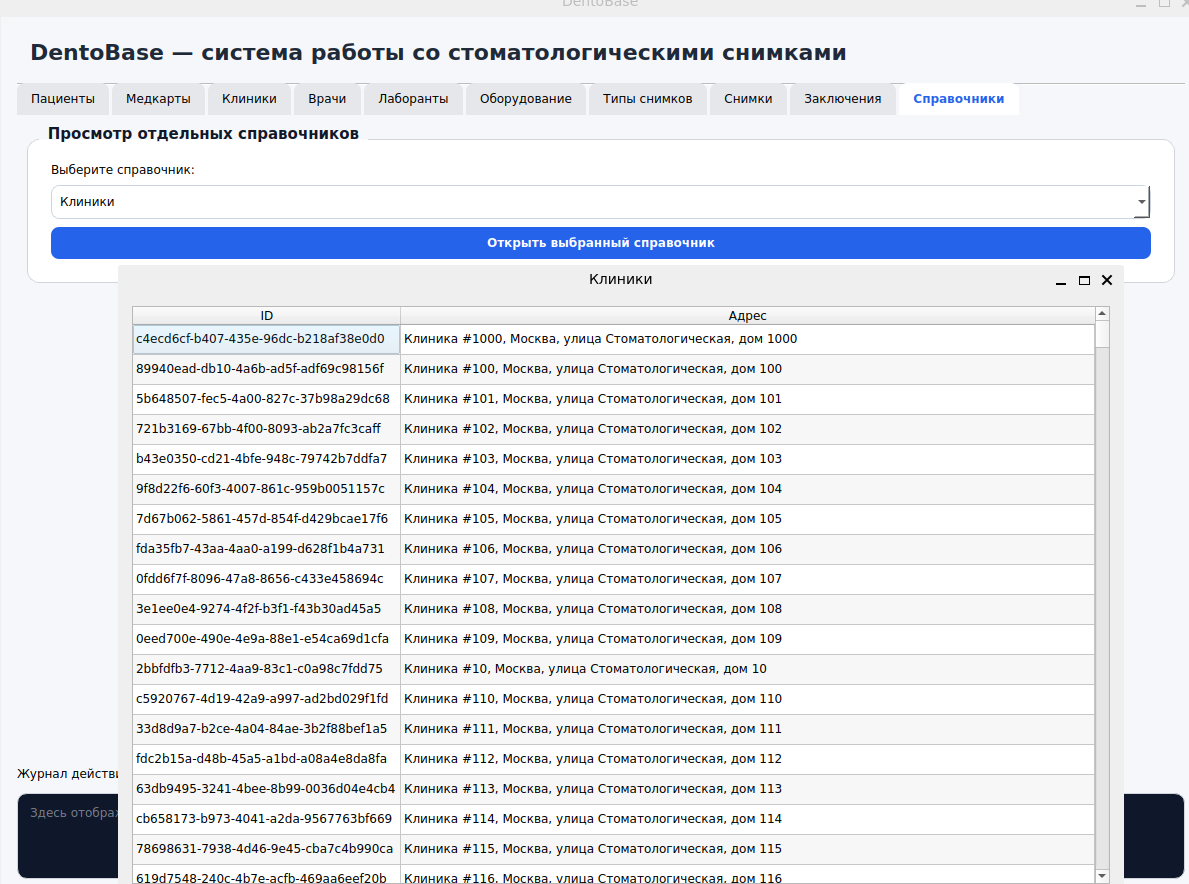
\includegraphics[width=0.7\textwidth]{graph2}
	\caption{Общий вид справочника}
	\label{fig:graph2}
\end{figure}

\begin{figure}[H]
	\centering
	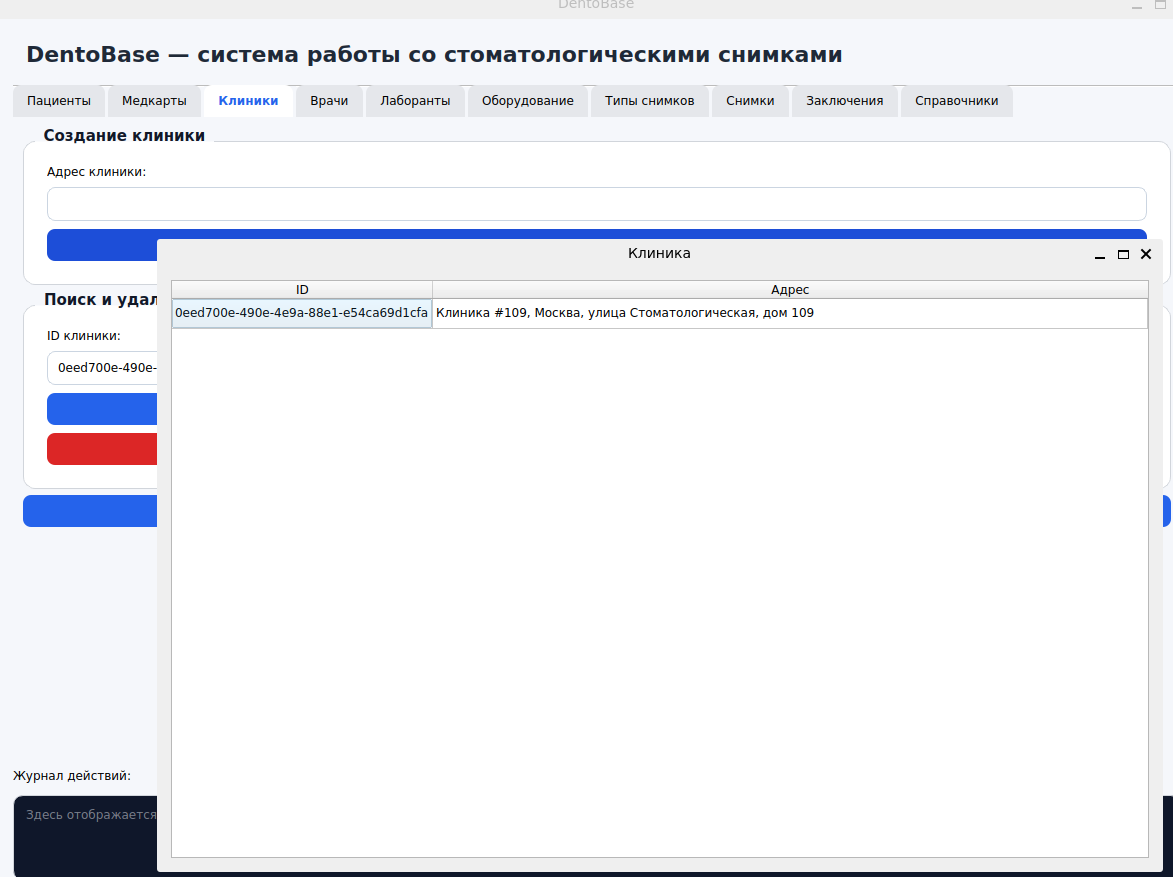
\includegraphics[width=0.7\textwidth]{graph3}
	\caption{Результат запроса}
	\label{fig:graph3}
\end{figure}

\begin{figure}[H]
	\centering
	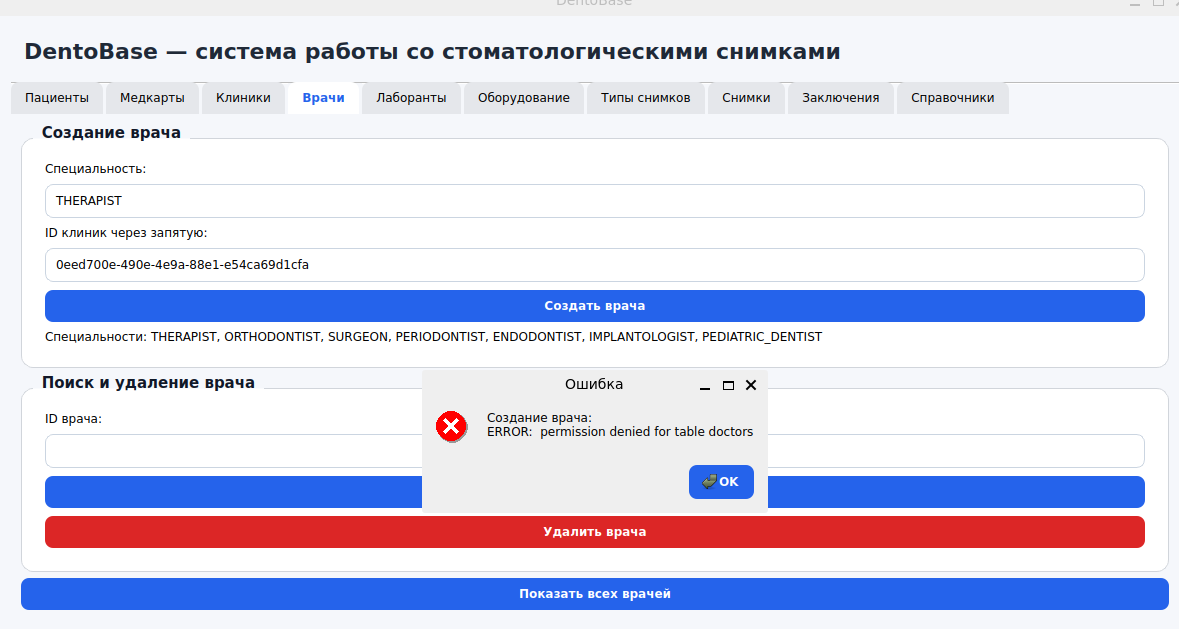
\includegraphics[width=0.7\textwidth]{graph4}
	\caption{Отказ в доступе}
	\label{fig:graph4}
\end{figure}

\section{Сборка проекта}

Сборка проекта выполняется с помощью CMake. Для сборки используются следующие команды:

\begin{lstlisting}[caption={Сборка проекта}]
	rm -rf build
	cmake -S . -B build
	cmake --build build
\end{lstlisting}

После сборки в директории \texttt{build/dist/components} формируются статические библиотеки компонентов:

\begin{itemize}
	\item \texttt{libdentobase\_config.a};
	\item \texttt{libdentobase\_logging.a};
	\item \texttt{libdentobase\_cache.a};
	\item \texttt{libdentobase\_data\_access.a};
	\item \texttt{libdentobase\_business.a};
	\item \texttt{libdentobase\_gui.a}.
\end{itemize}

Исполняемый файл графического приложения формируется в директории \texttt{build/dist} и имеет имя \texttt{dentobase\_gui\_app}.

\subsection{Запуск приложения}

Перед запуском приложения необходимо подготовить базу данных. Для этого используется скрипт:

\begin{lstlisting}[caption={Подготовка базы данных}]
	./scripts/reset.sh
\end{lstlisting}

После подготовки базы данных графическое приложение запускается командой:

\begin{lstlisting}[caption={Запуск графического приложения}]
	./build/dist/dentobase_gui_app config/admin.conf
\end{lstlisting}

Для запуска под другими ролями используются соответствующие конфигурационные файлы:

\begin{lstlisting}[caption={Запуск приложения под разными ролями}]
	./build/dist/dentobase_gui_app config/admin.conf
	./build/dist/dentobase_gui_app config/doctor.conf
	./build/dist/dentobase_gui_app config/technician.conf
\end{lstlisting}

\section{Тестирование приложения}

Для проверки корректности работы приложения были выполнены системные тесты через графический интерфейс. Тестирование включало проверку основных пользовательских сценариев и обработку ошибочных ситуаций.

Основные проверяемые сценарии:

\begin{itemize}
	\item создание пациента;
	\item поиск пациента;
	\item создание медицинской карты;
	\item создание и поиск клиники;
	\item создание и поиск врача;
	\item создание и поиск лаборанта;
	\item создание и поиск оборудования;
	\item создание и поиск типа снимка;
	\item загрузка снимка;
	\item создание заключения;
	\item удаление справочных сущностей;
	\item просмотр отдельных справочников;
	\item проверка записи логов;
	\item проверка Redis-кэширования;
	\item проверка ограничений ролевой модели.
\end{itemize}

Для проверки наполнения базы данных используется контроль количества записей после выполнения скрипта инициализации. Каждая основная таблица содержит не менее 1000 записей.

\begin{lstlisting}[caption={Проверка количества записей в таблицах}]
	SELECT 'patients' AS table_name, COUNT(*) FROM patients
	UNION ALL
	SELECT 'clinics', COUNT(*) FROM clinics
	UNION ALL
	SELECT 'doctors', COUNT(*) FROM doctors
	UNION ALL
	SELECT 'doctor_clinics', COUNT(*) FROM doctor_clinics
	UNION ALL
	SELECT 'technicians', COUNT(*) FROM technicians
	UNION ALL
	SELECT 'equipment', COUNT(*) FROM equipment
	UNION ALL
	SELECT 'image_types', COUNT(*) FROM image_types
	UNION ALL
	SELECT 'medical_records', COUNT(*) FROM medical_records
	UNION ALL
	SELECT 'images', COUNT(*) FROM images
	UNION ALL
	SELECT 'diagnoses', COUNT(*) FROM diagnoses;
\end{lstlisting}

\section*{Вывод}

В результате выполнения технологической части была реализована рабочая версия приложения DentoBase. Разработаны компоненты конфигурирования, логирования, кэширования, доступа к данным, бизнес-логики и графического интерфейса. База данных разворачивается автоматически с помощью скрипта, включающего создание схемы, функций, триггеров, тестовых данных и ролевой модели. Приложение поддерживает работу с PostgreSQL, Redis, ролевой моделью и графическим интерфейсом на Qt 6.